\subsection{Understanding neuronal response properties within the framework of NSC}

\jeffNote{MC 6: Box 3 needs to be re-written @Kris and @Emily. This is about the evolutionary framework, not the RSC. Describe CARLsim, how it interfaces with ECJ and the method we have on various datasets. Please include a figure (reproducing from one of our papers (Carlson et al., CARLsim 3 paper, or Rounds paper is fine). All those RSC details should go in the "Understanding neuronal response properties" section when describing the maze experiments}

% Spaghetti sentences...
Neuronal response properties can also be computed for model neurons with \ac{NSC}, which means that model neurons can be evaluated using methods similar to the ones employed by experimental researchers to understand biological neurons, and by theoretical neuroscientists to understand computational models. This is important because it means that NSC can be used to model neural activity in the brain, and the resulting activity patterns generated by NSC can be compared to and evaluated against experimental findings. 

% \jeffNote{make sure the nomenclature in the text agrees with the caption.  for example, neuron b in text and neuron h-bs in caption}


Neuronal response patterns can be computed by reconstructing the activity of a population of ``input'' neurons
(i.e., the $s$-th column in \textbf{V})
from a population of ``output'' neurons
(i.e., the $s$-th column in \textbf{H})
via their synaptic weights
(i.e., the matrix \textbf{W}; Fig.~\ref{fig:NMF|reconstruction}A).
Similarly, it is also possible to calculate \textbf{H} 
from $\mathbf{W^T}$ and \textbf{V}
(Fig.~\ref{fig:NMF|neuronalresponse}A).
In this context, a single element of \textbf{H} corresponds to the activity
of the $b$-th neuron to the $s$-th stimulus,
% of a particular model neuron $W_b$ to a particular stimulus $\vec{v}_s$,
which is given by the dot product of its presynaptic connections
(i.e., the $s$-th column in \textbf{V})
and the corresponding synaptic weights
(i.e., the $b$-th row in $\mathbf{W^T}$).
Note that the response of the model neuron to different stimuli 
$s \in 1, \ldots, S$
involves different columns of \textbf{H} and \textbf{V},
but always relies on the same weight matrix \textbf{W}.
Thus, we can utilize \textbf{W}
(which must remain fixed once learned with \ac{NMF})
to simulate a model neuron's response to arbitrary input stimuli
by replacing the column in \textbf{V} with new input.
This allows us to investigate the response properties of individual model neurons
much in the same way that experimental neuroscientists study biological neurons.
% \emilyNote{consistency in caption is still an issue for Fig 2. I don't know if $h_{bs}$ is right or not.}
% \mikeNote{Darn, A is wrong here, too. Should be the same column index in H as in V, either 3 or 4. To be consistent, should call H ``activity of output neurons'' and V ``activity of input neurons'' or similar, not neurons.}

\begin{figure}[h]
	\centering
	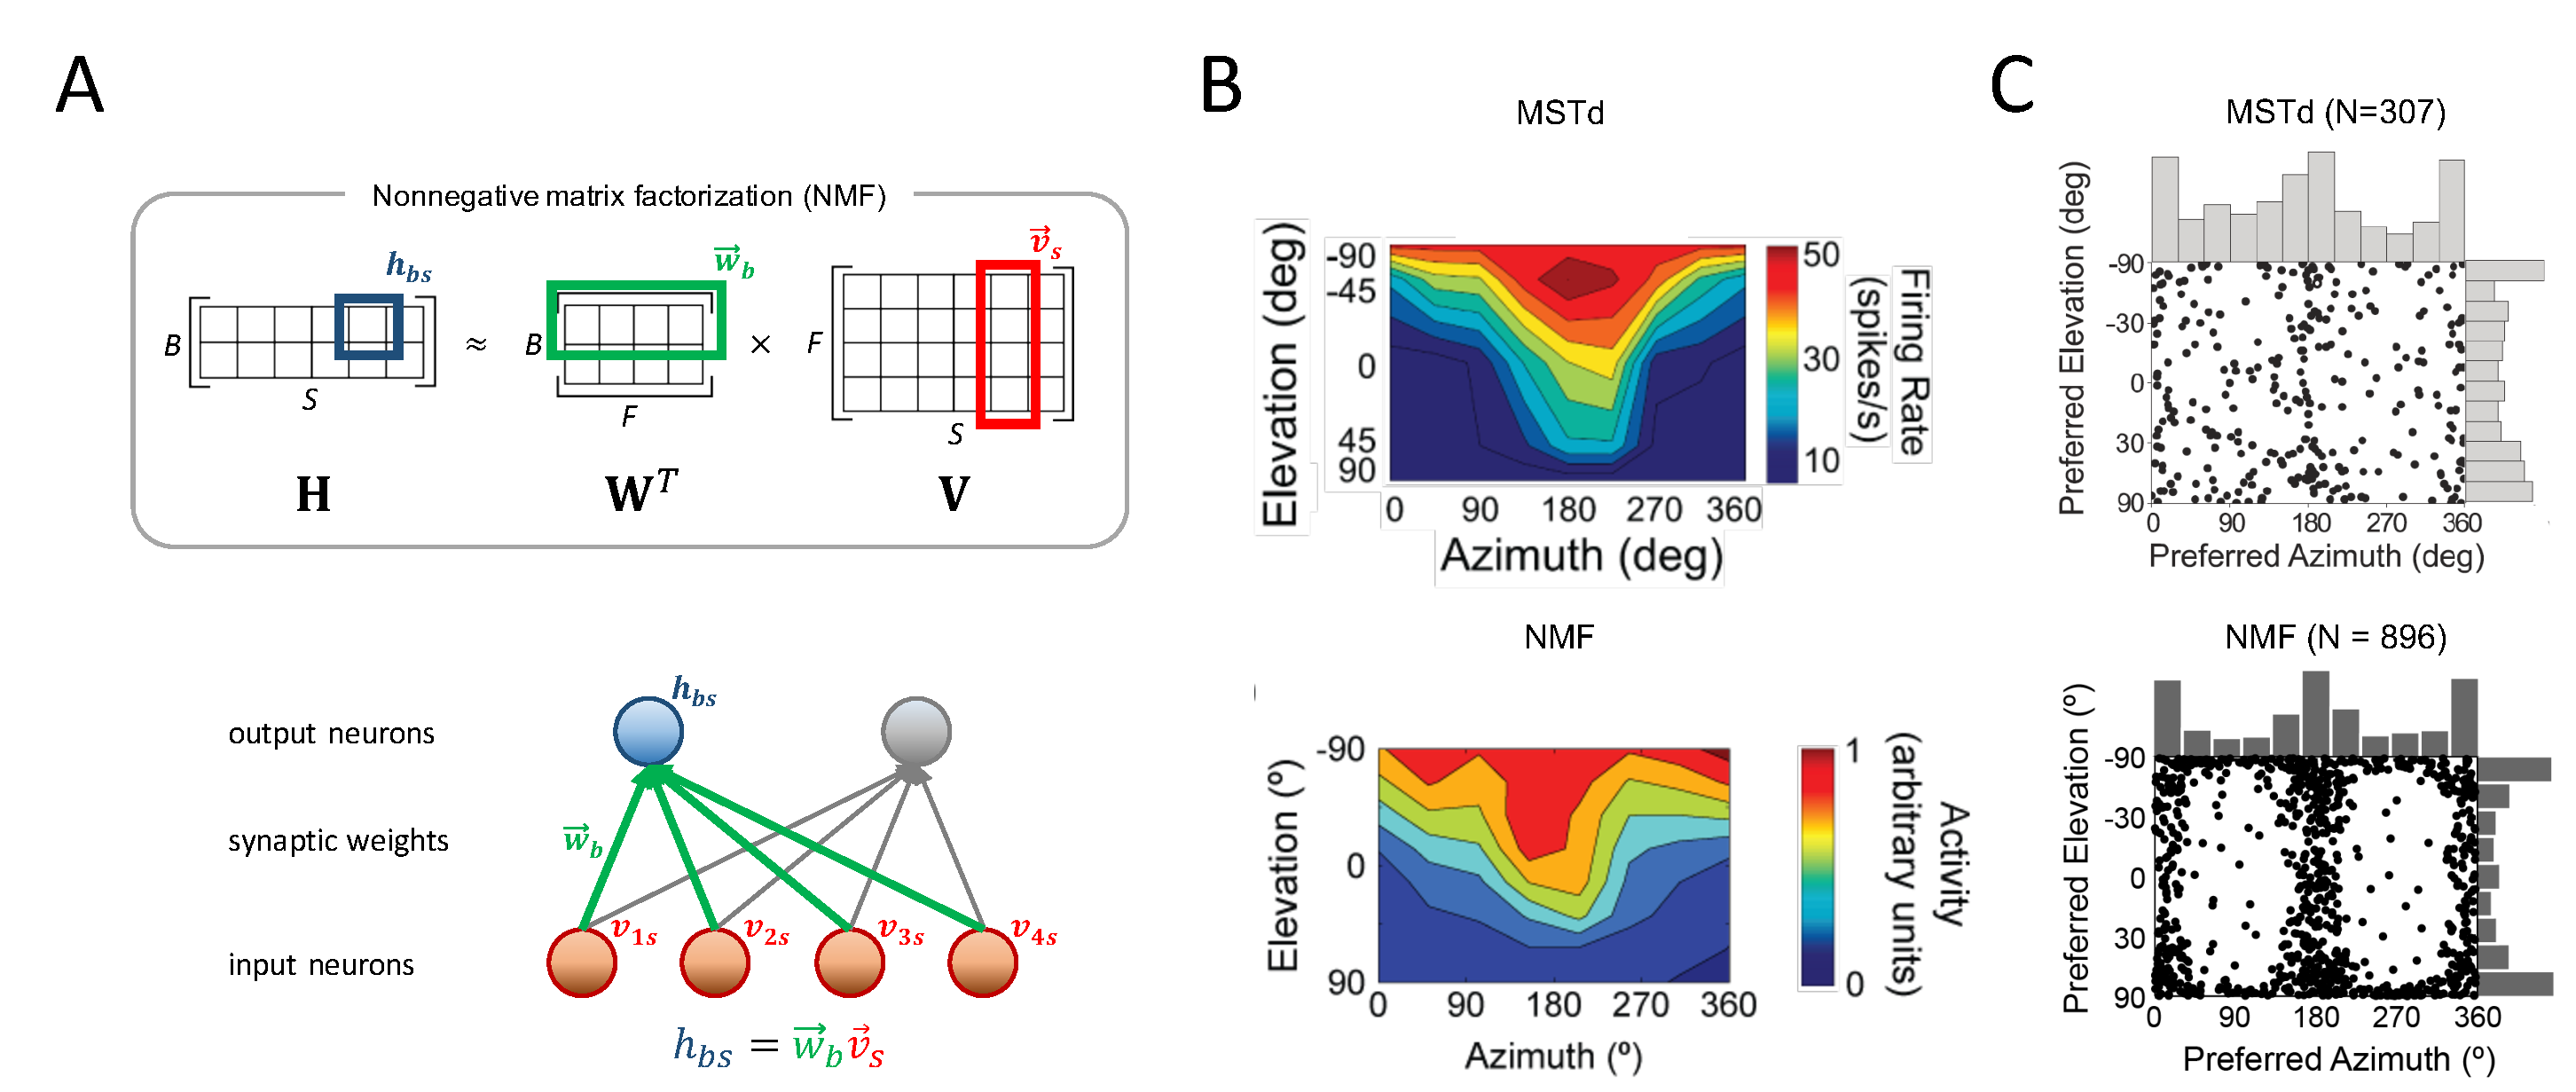
\includegraphics[width=\textwidth]{fig2_fixed}
    \caption{\ac{NSC} can predict response properties of biological neurons.
    A) Solving the \ac{NMF} equation for \textbf{H}, the response
       of output neuron $b$ to stimulus $s$ (i.e., matrix element
       $h_{bs}$) can be calculated from the activity of all
       input neurons (i.e., column $s$ in \textbf{V}) and the
       corresponding synaptic weights (i.e., row $b$ in
       $\mathbf{W}^T$).
    B) Example of 3D heading tuning for a neuron in macaque
       \ac{MSTd} (top, reprinted from \cite{Takahashi2007}) and a
       simulated neuron (bottom, reprinted from \cite{Beyeler2016}).
       Color contour maps show the mean firing rate or model
       activation as a function of azimuth and elevation angles
       of the self-movement direction in 3D.
    C) Classifying simulated akin to biological neuronal responses
       yields distributions of 3D heading preferences akin to 
       macaque \ac{MSTd} (top, reprinted from \cite{Beyeler2016}).
       Each neuron also responded to a preferred direction of 3D
       self-rotation (not shown).}
	\label{fig:NMF|neuronalresponse}
\end{figure}

\jeffNote{What is a Lambert cylindrical area?  Not needed to understand the figure. I deleted it.}
\mikeNote{Sounds good}

% Caption is currently 144 words
%Approximations of neuronal response patterns under NMF. (A) Top, neuronal response H can be approximated by multiplying the original input variable values by the basis functions W. Bottom, in an artificial neural network, the response of each neuron n is approximated by the product of the input neuron firing rates and the synaptic weights between each input neuron v and each hidden neuron h. (B) Top, something like ‘all population responses can be approximated by averaging across all neurons’ once we decide what goes there. Middle, neuron response profiles resulting from the application of NMF to MT-like inputs closely approximate the distribution of neuronal responses seen in biological MSTd. Bottom, response patterns resulting from the application of NMF to recorded behavioral variables encoded by idealized input neurons can be classified into categories that follow distributions similar to those seen in biological RSC data.


% \mikeNote{IMHO this comes all way too late in the narrative}
% The \ac{NSC} framework emerges naturally as a more biologically plausible
% extension of Olshausen and Field's sparse coding model \citep{OlshausenField1996}, which
% yielded features qualitatively similar to
% \acp{RF} of simple cells in \ac{V1}, but could not provide a literal interpretation for V1 simple-cell behavior given the lack of nonnegativity constraints on the inputs or units in the model \citep{Hoyer2003}.
% Hoyer observed that the matrices representing the input (\textbf{V}) and 
% output (\textbf{H}) neuronal activities should be restricted to positive values 
% \citep{Hoyer2003}, and logically concluded that the weights (\textbf{W}) should be constrained as well. Thus, the requirement of positive \textbf{V},
% \textbf{H}, and \textbf{W} matrix elements, along with the sparsity requirement from
% the original sparse coding model lead to the \ac{NSC} framework. 
% This seemingly simple fix had remarkable consequences on the quality of the
% sensory representation:
% Enforcing nonnegativity ensured that elementary image features combined additively
% (whereas in the standard sparse coding model features could
% ``cancel each other out'' through subtractive interactions),
% much like the intuitive notion of combining parts to form a whole.
% It should be noted that although the
% weights are restricted to positive values, inhibition still plays a role
% in inducing competition between output neurons and thus can be seen to motivate
% the sparseness constraint in equation 1 (Box 1).

%
% Should Figure 2 not mention STDP-H yet? I realize now that we're talking about it,
% it's kind of awkward to mention STDP-H since we haven't really talked about this yet.
% We could make Figure 2 just about experimental vs NMF

% Mike: Yes, Figure 2 should NOT have STDPH yet. That's only in Figure 3. 
% In fact, I don't see any STDPH stuff in Figure 2, which is good.


For example, subjecting model \ac{MSTd} neurons to simulated optic flow fields
mimicking natural viewing conditions during locomotion,
Beyeler and colleagues \citep{Beyeler2016} found that
individual model neurons
preferentially responded to a particular 3D direction of self-translation
and self-rotation,
much like individual neurons in macaque \ac{MSTd}
(Fig.~\ref{fig:NMF|neuronalresponse}B).
In addition, known statistical properties of the \ac{MSTd} population 
emerged naturally from the \ac{NMF} based model,
such as a relative over-representation of lateral headings (Fig.~\ref{fig:NMF|neuronalresponse}C).

% We next discuss a number of studies that are consistent with Hoyer\textsc{\char13}s
% interpretation, as they submit a hypothetical output neuron \textbf{h}
% to the same types of analysis as those performed by experimental neuroscientists.
% Carlson and colleagues \cite{Carlson2013} applied a temporal based learning rule
% to a simple model of V1 and found that the receptive fields of the output neurons
% encode orientation that qualitatively matched experiments in the cat \ac{V1}.
% Similarly, Beyeler and colleagues \citep{Beyeler2016} found that individual units
% in their model of \ac{MSTd} could signal the 3D direction of self-translation
% or self-rotation when presented with corresponding large-field motion stimuli.
% Not only did individual units match response properties of individual neurons
% in macaque \ac{MSTd},
% but the model was able to recover statistical properties of the \ac{MSTd}
% population as a whole, such as a relative overrepresentation of lateral
% headings (Fig.~\ref{fig:NMF|neuronalresponse}B).


%    In the case of the \ac{RSC}, the basis vectors that resulted from the NMF model produced activation patterns that could be used to infer behavior, suggesting that the model functions in a manner similar to the biological RSC. Because this region responds to multiple spatial frames of reference (egocentric, route-centric, and allocentric) simultaneously, it is possible to accurately reconstruct the position of an animal within a route situated in a specific part of the environment if neural activity for that route is compared with itself. In contrast, if neural activity associated with the same route but situated in different parts of the room are compared, then the reconstruction of position should be poor (for more details, see \citep{AlexanderNitz2015}), showing that the \ac{RSC} distinguishes routes that have different allocentric positions in space. We found that the activity patterns computed using the NMF basis vectors yielded qualitatively similar results when subjected to the same analysis.

% The results were also consistent for the \ac{RSC}. In the neurophysiological dataset, experimentally observed neurons were classified into three broad categories: 
% % these 3 are so incredibly, excruciatingly wordy 
% 1) those that were insensitive to turn-based actions performed by the rats running along the track but nonetheless exhibited complex and robust firing patterns, 2) those that were sensitive purely to turning behaviors performed by the rats such that they responded exclusively to left or right turns, and 3) neurons that demonstrated turn type selectivity, but with increased firing associated with specific instances of the preferred turn type based on their position in the turn sequence associated with the route regardless of the route's location in allocentric space. When \ac{NMF} was applied to the behavioral variables encoded by idealized input neurons, the resulting basis vectors could be categorized into the same functional categories and followed the same approximate distributions as in the experimental dataset (Fig.  \ref{fig:NMF|neuronalresponse}B).

Other groups have successfully applied methods similar to NSC to model neuronal response properties. For example, in the visual system, an NMF-based model was able to reconstruct neuronal spike trains in the salamander retina \citep{Onken2016}. Following testing on ground truth data, the researchers recorded spikes from in vitro retinal ganglion cells  while the cells were exposed to natural scenes (either still photographs or videos). They then applied several factorization methods to the data. Space-by-time NMF could decompose the data into separate spatial and temporal modules that yielded sparser and more compact representations compared to other techniques, including orthogonal Tucker-2 and basic NMF. \ac{NSC} could be used to reproduce response properties of \ac{V1} simple and complex cells \citep{HoyerHyvarinen2002,Hoyer2003} as well as V2 hypercomplex cells \citep{Hyvarinen2005}. Outside the visual stream, a model known as Reinforcement-Driven Dimensionality Reduction (RDDR) successfully used Hebbian learning to reproduce basal ganglia response patterns associated with reward \citep{BarGad2000}, a function associated with cortico-striato-pallidal circuitry. The authors later applied nonnegativity constraints to the Hebbian learning in the model so that it performed \ac{NMF} on its inputs. The model advanced understanding of the cortico-striato-pallidal loop by capturing behavior of the circuit while explaining the existence of convergent and lateral connections in the region that other models have historically ignored \citep{BarGad2003_Review}. The authors suggest that the basal ganglia uses unsupervised, reward-driven learning to perform dimensionality reduction on cortical inputs for the efficient compression of information in order to plan upcoming actions in the frontal cortex.


% In the visual system,
% an \ac{NMF} based model was able to reconstruct
% neuronal spike trains in the salamander retina \citep{Onken2016},
% and \ac{NSC} could be used to reproduce response properties
% of \ac{V1} simple and complex cells \citep{HoyerHyvarinen2002,Hoyer2003} as well as V2 hypercomplex cells \citep{Hyvarinen2005}.


% NMF can also describe patterns of activation observed in retinal ganglion cells (RGCs), which exhibit specific response times and latencies in response to natural images that allow the retina to encode spatial and temporal information embedded in the stimuli. A specific form of NMF, called Tucker-2 or space-by-time NMF, produces separate spatial and temporal basis vectors that most accurately and sparsely describe the spike trains produced by RGCs in the salamander retina \citep{Onken2016}. Nonnegativity constraints, possibly in conjunction with other statistical constraints dependent on the brain region the neurons operate in, may describe the response patterns of neurons in other brain regions that have yet to be tested.



% I feel like I haven't described this clearly but I'm trying to be concise...
% Mike: I feel like this is to complicated to bring up, I'd say cut it...

% In the case of the \ac{RSC}, the basis vectors that resulted from the NMF model produced activation patterns that could be used to infer behavior, suggesting that the model functions in a manner similar to the biological RSC. Because this region responds to multiple spatial frames of reference (egocentric, route-centric, and allocentric) simultaneously, it is possible to accurately reconstruct the position of an animal within a route situated in a specific part of the environment if neural activity for that route is compared with itself. In contrast, if neural activity associated with the same route but situated in different parts of the room are compared, then the reconstruction of position should be poor (for more details, see \citep{AlexanderNitz2015}), showing that the \ac{RSC} distinguishes routes that have different allocentric positions in space. We found that the activity patterns computed using the NMF basis vectors yielded qualitatively similar results when subjected to the same analysis.

The finding that \ac{NSC} can account for neuronal response properties across
brain areas and modalities supports the view that these 
preferences emerge from the pressure to find efficient representations
of perceptually or behaviorally relevant stimulus spaces.
At the population level, \ac{NSC} promotes representations in which
neurons act as generalists rather than specialists,
allowing for the simultaneous encoding of multiple variables of interest
(e.g., heading, eye rotation velocity in \ac{MSTd} \citep{Beyeler2016})
with respect to multiple frames of reference
(e.g., egocentric, route-based in \ac{RSC} \citep{Rounds2016}).
Among the advantages of such basis function representations
\citep{Poggio1990,PougetSejnowski1997,PougetSnyder2000}
(also called mixed-selectivity representations
\citep{Eichenbaum2017,Fusi2016,Barak2013})
are robustness to noise as well as the ability to decode various variables of interest
by taking a linear combination of neuronal responses.
\jeffNote{A couple times you used the term "hard-wired neuronal specificity". This doesn't make sense in this context. All the NSC examples are hard-wired. Even STDPH is technically hard-wired.}

% The fact that  \ac{NSC} can account for the response properties of neurons in a diverse set of brain regions that play fundamentally different roles in behavior and cognition is somewhat astounding since individual brain regions are often assumed to have their own unique methods of handling their unique inputs. Evidence for the prevalence of such a computation raises some fundamental questions about how neurons have evolved to help us survive. In particular, these findings suggest that neurons are not, in fact, specialized for particular kinds of computations or functionality, and that it is more advantageous for neurons to be capable of handling all information flexibly. Several researchers have argued that 'mixed selectivity' is a fundamental feature of neurons in higher cortical regions \citep{Eichenbaum2017,Fusi2016,Barak2013}, because higher cognition requires that neurons encode multiple task-relevant variables. Such generalizability is an expected property of neurons under the NSC framework, since the algorithm aims to encode as much information about the stimulus as possible while using the fewest number of neurons to do it. If optimizing these metrics, it is expected that neurons would not be specialized for certain behaviors or inputs, and would instead be equally likely to respond to all types of inputs. This is further supported by evidence showing that sparsity levels amidst populations of neurons demonstrating mixed selectivity helps to control the tradeoff between generalization and discrimination \citep{Barak2013}.

% Another really important finding: Why sparsity? Turns out sparsity is what keeps mixed-selectivity neurons from overgeneralizing. Sparsity levels control generalization-discrimination trade off.
% Mike - ref?

% The fact that \ac{NSC} can reproduce all these response properties is mind-blowing,
% isn't it.
% These findings raise the possibility that certain stereotypical 
% neuronal response properties
% are not hard-wired
% to support a particular function,
% perhaps because the function is behaviorally relevant.
% Instead, these responses might simply emerge as a by-product
% of neuron's performing dimensionality reduction on their inputs.
% \mikeNote{Add some point we should make the following remark}
% This could explain all the mixed-selectivity neurons
% (e.g., if you engineer a system for navigation,
% there's no obvious reason to have a multi-tasking RSC neuron).
% But in the framework of \ac{NSC} it makes sense, because you want neurons that
% act like basis functions - neurons that are generalists instead of specialists.
% good, we can cite that fusi paper now


